\documentclass[14pt]{beamer}
\title[CP01.13 BC]{JEE :: Advanced JDBC}
\author[TS]{TalentSprint}
\institute[L\&D]{Licensed To Skill}
\date{Version 1.0.4}
\usefonttheme{serif}
\usecolortheme{orchid}
\usepackage{bookman}
\usepackage{hyperref}
\usepackage[T1]{fontenc}
\usepackage{graphicx}
\usepackage{listings}
\usepackage{multicol}
\graphicspath{{../../Images/}}
\lstset{language=Java,numbers=left, numberstyle=\tiny, basicstyle=\footnotesize, numbersep=10pt, showstringspaces=false, breaklines=true,keepspaces=true, columns=flexible}
\beamertemplateballitem
\usebackgroundtemplate{
\includegraphics[width=\paperwidth]{TS-Logo.jpg}}

\begin{document}
\begin{frame}
  \titlepage
\end{frame}

\begin{frame}{Advanced JDBC}
The content in this presentation is aimed at teaching  learners to:
\begin{itemize}
  \item Operations performed by database engine
  \item Programming interaction on Statement interface
  \item Flow of Statement interface working
  \item Problems with Statement interface
\end{itemize}
\end{frame}

\begin{frame}{Advanced JDBC}
The content in this presentation is aimed at teaching  learners to:
\begin{itemize}
  \item Understanding PreparedStatement
  \item Flow of PreparedStatement working
  \item Programming Interaction
\end{itemize}
\end{frame}


\begin{frame}{Advanced JDBC}
\textbf{Operations Performed By Database Engine}
\begin{itemize}
\item Most databases handles JDBC/Sql Query in four steps
\begin{itemize}
\item Parse the incoming query.
\item Parse the incoming query.
\item Optimize the data path.
\item Execute the optimized query to acquire and return data
\end{itemize}
\item In JDBC, Statement interface and it's sub interface known as PreparedStatement interface are used to query the database.
\end{itemize}

\end{frame}


\begin{frame}[fragile]{Advanced JDBC}
\textbf{Statement Interface Example}
\begin{lstlisting}[numbers=none]
import java.sql.*;
public class JDBCExample {
    public static void main(String[] args) {
        Connection conn = null;
        Statement stmt = null;
        String sql=””;
        try{
            //STEP 2: Register JDBC driver
            Class.forName("com.mysql.jdbc.Driver");
            conn = DriverManager.getConnection(“jdbc:mysql://localhost:3306/mysql”, USER, PASS);
            stmt = conn.createStatement();
\end{lstlisting}
\end{frame}
\begin{frame}[fragile]{Advanced JDBC}
\begin{lstlisting}[numbers=none]
            sql = "INSERT INTO Registration VALUES (100, 'Veer',19)";   
            stmt.executeUpdate(sql);
            sql = "INSERT INTO Registration VALUES (101, 'Zara', 18)";
            stmt.executeUpdate(sql);
            System.out.println("Inserted records into the table...");
        }
        catch(SQLException se) {
            //Handle errors for JDBC
            se.printStackTrace();
        }
        catch(Exception e) {
            //Handle errors for Class.forName
            e.printStackTrace();
        }
    }
}
\end{lstlisting}
\end{frame}

\begin{frame}{Advanced JDBC}
\textbf{Working of Statement Interface}
Let us understand how Statement interface is working
\begin{center}
    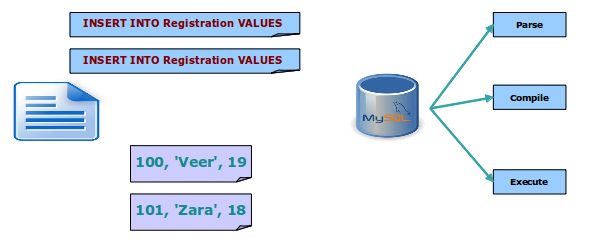
\includegraphics[scale=0.5]{JEE-M03-S02-Image1.png}
  \end{center}
It is clear now for every new statement database has to do parsing, compiling and executing operations always.
\end{frame}

\begin{frame}{Advanced JDBC}
\textbf{Problems With Statement Interface}
\begin{itemize}
\item Database parses the same query multiple times, executes and fetches the result.
\item All four steps that is parsing, compiling, optimizing, fetching are always repeated.
\item Network traffic to the Database is heavy since same query goes multiple times.
\item To overcome this problem we have to use precompiled statements.
\end{itemize}
\end{frame}


\begin{frame}{Advanced JDBC}
\textbf{PreparedStatement}
\begin{itemize}
\item It is inherited from Statement interface.
\item In database management systems, a prepared statement or parameterized statement is a feature used to execute the same or similar database statements repeatedly with high efficiency
\item It pre-executes parsing, compiling, optimizing. Thus, when creating PreparedStatement some optimization is done immediately.
\end{itemize}
\end{frame}


\begin{frame}{Advanced JDBC}
\textbf{PreparedStatement}
\begin{itemize}
\item The statement template is created by the application and sent to the database management system (DBMS). Certain values are left unspecified, called parameters, placeholders or bind variables (labelled ``?'' below):

\end{itemize}
\begin{center}
    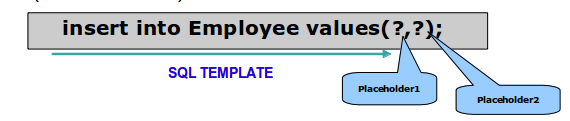
\includegraphics[scale=0.5]{JEE-M03-S02-Image2.png}
  \end{center}
\end{frame}


\begin{frame}{Advanced JDBC}
\textbf{PreparedStatement Working}
\begin{center}
    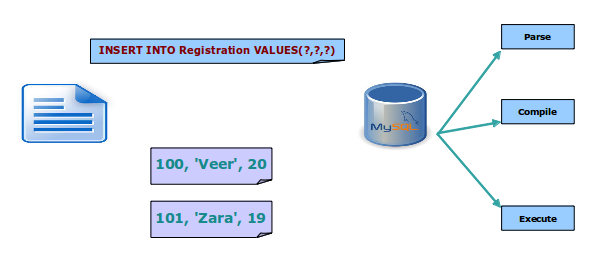
\includegraphics[scale=0.5]{JEE-M03-S02-Image3.png}
  \end{center}
As we could see that PreparedStatement is parsed and compiled only once and execute many times using new values.
\end{frame}

\begin{frame}{Advanced JDBC}
\textbf{PreparedStatement Interface}
\begin{center}
    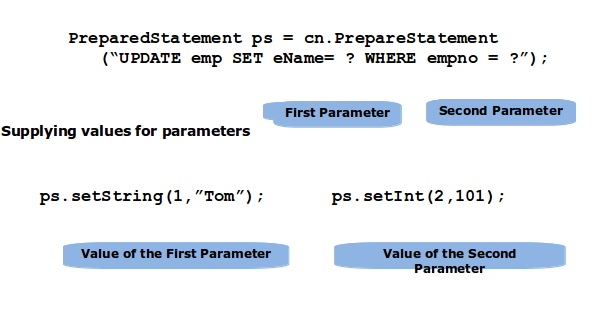
\includegraphics[scale=0.5]{JEE-M03-S02-Image4.png}
  \end{center}

\end{frame}

\begin{frame}{Advanced JDBC}
\textbf{Rules to Remeber}
\begin{center}
    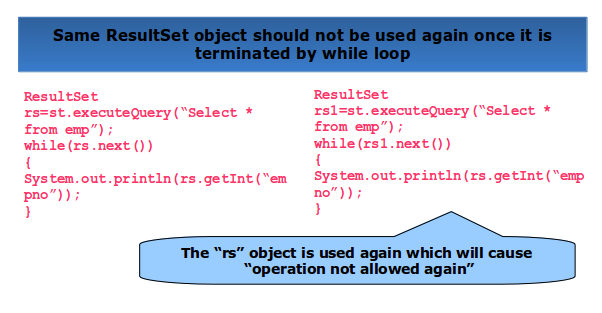
\includegraphics[scale=0.5]{JEE-M03-S02-Image5.png}
  \end{center}

\end{frame}

\begin{frame}{Advanced JDBC}
\textbf{Rules to Remeber}
\begin{center}
    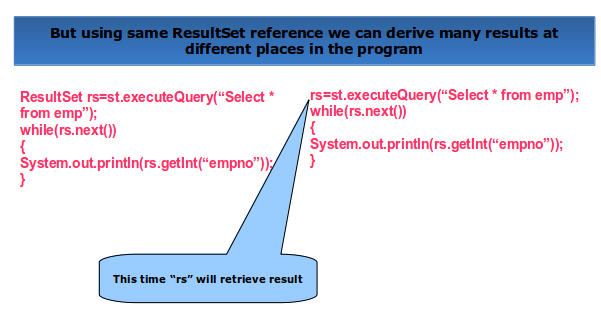
\includegraphics[scale=0.5]{JEE-M03-S02-Image6.png}
  \end{center}

\end{frame}

\begin{frame}{Advanced JDBC}
\begin{center}
    
\includegraphics[scale=0.5]{QA.png}
  \end{center}

\end{frame}
\end{document}
